\documentclass[12pt, a4paper]{article}
\usepackage[utf8]{inputenc}
%\usepackage[IL2]{fontenc}
\usepackage[czech]{babel}
\usepackage[pdftex]{graphicx}
\usepackage{mathtools}
\usepackage{amsmath}
\usepackage{svg}
\usepackage{textcomp}
\usepackage{listings,xcolor}
\usepackage[final]{pdfpages}
\usepackage{verbatim}
\usepackage{fancyhdr}
\usepackage[T1]{fontenc}

\usepackage[nottoc,notlot,notlof]{tocbibind}
\usepackage[pdftex,hypertexnames=false]{hyperref}
\hypersetup{colorlinks=true,
  unicode=true,
  linkcolor=black,
  citecolor=black,
  urlcolor=black,
  bookmarksopen=true}

\title{\textbf{Dokumentace semestrální práce} \\KIV/NET}
\author{Vojtěch Danišík}
\begin{document}

\begin{titlepage} 
	\newcommand{\HRule}{\rule{\linewidth}{0.5mm}} 
	\begin{center}
	
\includegraphics[width=12cm]{img/fav_logo}\\
	\end{center}
	\textsc{\LARGE Západočeská univerzita v Plzni}\\[1.5cm] 	
	\textsc{\Large Programování v prostředí .NET}\\[0.5cm] 
	\textsc{\large KIV/NET}\\[0.5cm] 
	\HRule\\[0.4cm]
	{\huge\bfseries Zpracování naměřených teplot}\\[0.4cm] 
	\HRule\\[1.5cm]
	
	\begin{minipage}{0.4\textwidth}
		\begin{flushleft}
			\large
			Vojtěch \textsc{Danišík}\newline
			A19N0028P\newline
			danisik@students.zcu.cz
		\end{flushleft}
	\end{minipage}
	\vfill\vfill\vfill
	\begin{flushright}
	{\large\today}
	\end{flushright}
	\vfill 
\end{titlepage}

\newpage
Souhlasím s vystavením této semestrální práce na stránkách katedry \newline informatiky a výpočetní techniky a jejímu využití pro prezentaci pracoviště.
\newline
\begin{flushright}
Vojtěch Danišík
\end{flushright}

\newpage
\tableofcontents

\newpage
\section{Zadání}
Desktopová aplikace v programovacím jazyce C\#, která umožňuje zaznamenat naměřené teploty ve městech za daný měsíc. Cílem aplikace je možnost zaznamenat si naměřené teploty za daný měsíc pro určité město v daný rok. Zaznamenané teploty se poté zprůměrují v daný měsíc a lze si následně vykreslit 3 grafy:
\begin{itemize}
\item Průměrná teplota ve všech městech po měsíci v daný rok.
\item Porovnání teplot více měst po měsících v daný rok.
\item Teplota ve městech za měsíc v daný rok.
\end{itemize}
V aplikaci si uživatel bude moct zvolit jednotku teploty. Zvolená jednotka teploty bude aplikována na data v aktuálně zpracovávaném roce. Na výběr budou 3 jednotky:
\begin{itemize}
\item Stupeň Fahrenheita [°F]
\item Stupeň Celsia [°C]
\item Kelvin [K]
\end{itemize}
Aplikace bude umožňovat přidávání / mazání měst, přidávání / mazání jednotek teplot a přidávání / mazání sestav. Aplikace dále umožní zaznamenané teploty v daný rok exportovat do csv.

\newpage
\section{Analýza}
\subsection{Windows Forms}
Windows Forms je open-source grafická knihovna, která je součástí .NET Core UI frameworku a slouží pro vytváření desktopových aplikací pro Windows. Je to předchůdce WPF.

Ve Windows Form se programuje pomocí takzvaného \textbf{event-driven programming}, což znamená, že běh programu je určen událostmi, jako například uživatelské události (kliknutí myši, zmáčknutí tlačítka), nebo zprávami od ostatních programů nebo vláken. Aplikace jako taková stráví většinu času čekáním na události.

Pro vytváření aplikací se využívá \textbf{visual designer}, pomocí kterých si uživatel na předem vytvořené okno může vkládat různé vizuální prvky (tlačítko, textové pole), kterým lze nastavit i různé události (například Drag \& Drop události).

\subsection{Databáze}
V aplikaci byla použita Service-based databáze. Service-based databáze je databáze, ke které se lze připojit pouze přes Microsoft SQL Server a využívá datový formát MDF (SQL Server formát). Pro připojení do databáze je potřeba mít řetězec pro připojení do databáze (\textit{Connection string}, viz příklad \ref{eq:connection_string}) a server musí běžet.

\begin{equation}
\begin{split}
Data Source=(LocalDB)/MSSQLLocalDB; \\
AttachDbFilename=|DataDirectory|/Database.mdf; \\
Integrated Security=True
\end{split}
\label{eq:connection_string} 
\end{equation}

Pro vytvoření spojení mezi aplikací a serverem se následně používá knihovna \textit{System.Data.SqlClient}, které se zadá \textit{connection string} a ta nám vytvoří dané připojení. Přislušná knihovna se stahuje pomocí NuGet balíčkovacího systému pro daný projekt.

V databázi se nachází 4 tabulky (viz ERA model na obrázku \ref{fig:era_model}):
\begin{itemize}
\item \textbf{Measure} - V tabulce se nachází názvy a symboly jednotek teplot, které se budou používat u jednotlivých datasetů. Každý dataset může používat pouze jednu jednotku teploty.
\item \textbf{Dataset} - Záznamy v této tabulce reprezentují seznam záznamů za daný rok. V každém záznamu bude použita přiřazená jednotka teploty.
\item \textbf{City} - V tabulce se nachází názvy měst, které lze použít ve všech datasetech.
\item \textbf{Record} - Jeden záznam, který reprezentuje seznam teplot v daném městě za celý rok. Záznam je vždy přiřazen k jednomu datasetu.
\end{itemize}
\begin{figure}[h!]
	\centering
	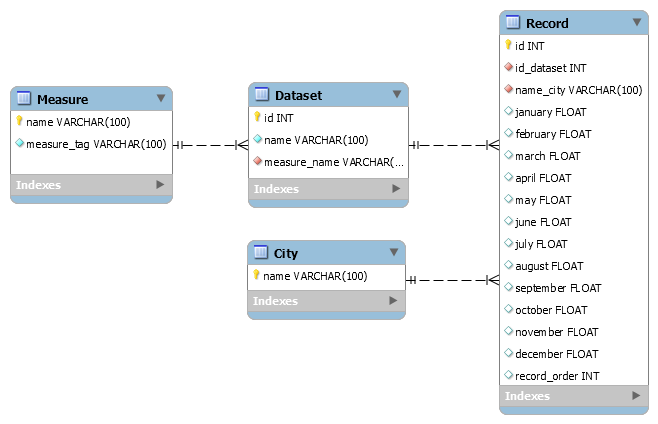
\includegraphics[width=12cm]{img/era.png}
	\caption{ERA model}
	\label{fig:era_model}	
\end{figure}

\newpage
\section{Implementace}
Aplikace se skládá ze tří hlavních vrstev - Datová, Modelová a Prezentační. V aplikaci byla použita lokální databáze, která se nachází ve stejném adresáři jako výsledná aplikace.
\subsection{Datová vrstva}
Datová vrstva je řesená jako samostatná knihovna (Class library), která se připojuje k modelové a prezentační vrstvě. Datová vrstva obsahuje třídy, které reprezentují tabulky v databázi, a také výčtové typy pro grafy. ERA model databáze lze vidět na obrázku \ref{fig:era_model}.

\subsection{Modelová vrstva}
Modelová vrstva je řešená jako samostatná knihovna (Class library) a je závislá na datové vrstvě. Modelová vrstva obsahuje interface k připojené databázi, pomocí kterého lze získat data z databáze pomocí předem připravených metod. Tyto metody obsahují předpřipravené SQL dotazy. Do dotazů jsou přidávány parametry pomocí třídy \textbf{SqlParameter}, která zabezpečuje přenos dat proti SQL Injection.

V modelové vrstvě se také nachází jednotlivý manažeři ke všem vytvořeným oknům v prezentační vrstvě, pomocí kterých lze získat data z interface databáze.

\subsection{Prezentační vrstva}
V prezentační vrstvě se nachází veškeré GUI prvky aplikace a 5 oken, pomocí kterých lze spravovat a zobrazovat uložené záznamy. Velikost oken je pevně daná, nelze je nijak zvětšovat / zmenšovat.
\subsubsection{Vlastní GUI elementy}
V aplikaci bylo potřeba změnit 3 základní GUI prvky (všechny jsou součástí prvku \textit{DataGridView}) :
\begin{itemize}
\item \textbf{CityCell} - Rozšíření třídy \textit{DataGridViewComboBoxCell} o textový atribut, který obsahuje název zvoleného města u záznamu v tabulce aplikace.
\item \textbf{MonthCell} - Rozšíření třídy \textit{DataGridViewTextBoxCell}  o 2 atributy. První atribut je číslo v plovoucí čárce, které reprezentuje hodnotu teploty v daném měsíci. Druhý atribut je textový řetězec, který obsahuje zvolenou jednotku teploty pro hodnotu. Tyto atributy byly potřeba, aby se při nezvolené buňce zobrazovala hodnota i s jednotkou teploty, zatímco při zvolení dané buňky se jednotka teploty vymaže z textového pole.
\item \textbf{DataGridViewRowWithId} - Rozšíření třídy \textit{DataGridViewRow} o ID atribut řádku, aby bylo mazání / přidávání / upravování záznamů v tabulce snažší.
\end{itemize}

\subsubsection{Hlavní okno}
Hlavní okno aplikace, ve kterém lze zobrazovat / upravovat záznamy ve zvolených datasetech a otevírat všechna ostatní okna. 
\begin{itemize}
\item Zobrazení záznamů v \textit{DataGridView} proběhne ihned po zvolení daného datasetu ze seznamu datasetů.
\item Každý záznam obsahuje jeden \textbf{CityCell} pro výběr města, ve kterém se teploty zaznamenaly, a 12 \textbf{MonthCell} pro zaznamenání teploty v daném měsíci. Každá buňka pro měsíc obsahuje validátor vstupu, který povoluje pouze mínus, čárku a číslice. Vložená hodnota teploty je ještě zvalidována, zda text je zformátován jako celé nebo desetinné číslo.
\item Každá zaznamenaná změna v datasetu nastaví příznak \textbf{recordsChanged}, který určuje, zda byl seznam recordů změněn (změna hodnot v existujícím záznamu, smazání / přidání nového záznamu). Ten se využívá při otevírání okna s grafama / otevírání nového datasetu / exportu dat do CSV, kdy aplikace zobrazí info hlášku, že aktuální dataset byl změněn.
\item Pořadí záznamů lze měnit pomocí přetáhnutím daného záznamu na jinou pozici (Drag \& Drop), nebo kliknutím na sloupec v tabulce, který dané záznamy vyfiltruje podle abecedy (u měst) nebo podle číselných hodnot (u teplot v měsíci).
\end{itemize}
Při exportu záznamů z aktuálně zvoleného datasetu se používá \textbf{SaveFileDialog}, který přednastaví příponu souboru na CSV. Jednotlivé hodnoty v záznamu jsou odděleny středníkem.

\subsubsection{Okno pro správu měst}
 Okno pro správu názvů měst v databázi. V okně se nachází \textit{DataGridView} obsahující veškeré názvy měst v databázi a tlačítka, pomocí kterých lze přidávat / mazat města z tabulky. V \textit{DataGridView} lze označovat více položek najednou.

Město se z databáze smaže tehdy, pokud se město nenachází v žádném záznamu v kterémkoliv datasetu (kontrola probíhá pomocí SQL dotazu).

\subsubsection{Okno pro správu teplot}
Okno pro správu jednotek teplot v databázi. V okně se nachází \textit{DataGridView} obsahující všechny vytvořené jednotky teploty i s jejich symbolem. Zároveň jsou zde tlačítka, pomocí kterých lze přidávat / mazat / upravovat jednotky teploty v tabulce. V \textit{DataGridView} lze označovat více položek najednou.

Jednotka teploty se z databáze smaže tehdy, pokud není použita v žádném datasetu (kontrola probíhá pomocí SQL dotazu). Symbol jednotky teploty může být měněn kdykoliv.

\subsubsection{Okno pro správu datasetů}
Okno pro správu datasetů v databázi. V okně se nachází \textit{DataGridView} obsahující všechny vytvořené datasety a jim přiřazené jednotky teploty pro jednotlivé záznamy. Zároveň jsou zde tlačítka, pomocí kterých lze přidávat / mazat / upravovat datasety v tabulce. V \textit{DataGridView} lze označovat více položek najednou.

Při mazání datasetu se rovnou provede smazání všech záznamů v tabulce \textbf{Record}, kteří jsou přiřazeny danému datasetu. Pokud byl v hlavním okně smazám vybraný dataset, tak aplikace vyhodí upozorňující zprávu, že aktuálně vybraný dataset byl smazán a bude vybrán první dataset (pokud nějaký existuje).

\subsubsection{Okno s grafy}
Okno, ve kterém lze zobrazit předdefinované typy grafů. V okně se nachází 2 \textit{ComboBoxy}, pomocí kterých si lze vybrat typ grafu a dataset, ze kterého budou čerpána data. Pro zobrazení dat v grafu je zde použit \textit{ChartArea}. Vykreslená data obsahují i tooltip texty pro přesnější vyobrazení dat a legendu. Také se zde nachází \textit{ListBox}, který v některých případech obsahuje volitelné položky, které jsou potřeba u některých typů dat:
\begin{itemize}
\item \textbf{Průměrná teplota ve všech městech po měsíci v daný rok} - Žádná dodatečné informace nejsou potřeba, graf se rovnou vykreslí. Na X-ové ose se nachází všechny měsíce, na Y-ové ose jsou zprůměrované hodnoty teplot ve všech městech v datasetu. 
\item \textbf{Porovnání teplot více měst po měsících v daný rok} - V listboxu se zobrazí všechna města použitá v daném datasetu. Po kliknutí na jakékoliv město (lze vybrat více měst) se ihned zobrazí graf. Na X-ové ose se nachází všechny měsíce, na Y-ové ose jsou hodnoty teplot v daném městě (jednotlivé záznamy teplot  jsou odděleny barvou specifickou pro dané město, které je zobrazeno v legendě grafu).
\item \textbf{Teplota ve městech za měsíc v daný rok} - V listboxu se zobrazí měsíce, kdy lze zvolit pouze jeden měsíc. Po zvolení měsíce se graf ihned zobrazí. Na X-ové ose se nachází všechna města v datasetu, na Y-ové ose jsou hodnoty teplot pro dané město.
\end{itemize}

V každém grafu se nachází titulek, který se skládá z názvu typu grafu a názvu zvoleného datasetu. Y-ová osa má nastavené minimum a maximum, kdy minimum se rovná nejmenší hodnotě, která bude v grafu zobrazena, a maximum se rovná největší hodnotě, která bude v grafu zobrazena, ke které se přičtě hodnota 2 pro lepší zobrazení dat.

\newpage
\section{Uživatelská příručka}
V aplikaci se nachází 5 oken. Hlavní okno se otevře při zapnutí aplikace a jeho vzhled lze vidět na obrázku \ref{fig:main_window}. 

\subsection{Hlavní okno}
V hlavním okně si lze vybrat jeden z mnoha datasetů. Po vybrání jakéhokoliv datasetu se zobrazí veškeré záznamy přiřazené k danému datasetu. Pod vybraným datasetem se zobrazí vybraná jednotka teploty.

Pro přidání nové řádky je potřeba kliknout na tlačítko "\textbf{Přidat řádku}". Nová řádka nebude mít vybrané žádné město a všechny hodnoty budou nastaveny na hodnotu 0. U nové řádky je potřeba zvolit město, které se nenachází v žádném záznamu.

Pro smazání jedné nebo více řádek je potřeba označit dané řádky pomocí levého tlačítka (ctrl + levé tlačítko pro výběr více řádků) a kliknout na tlačítko "\textbf{Odebrat označené řádky}".

Pokud se provede změna u kteréhokoliv záznamu / přidá se nový záznam, je potřeba tyto změny uložit do databáze. Pro potvrzení / zahození změn stačí kliknout na tlačítko "\textbf{Potvrdit změny}" / "\textbf{Zrušit změny}", které se nacházejí v levém dolním rohu hlavního okna.

V pravém dolním rohu se nachází tlačítko pro export aktuálně vybraného datasetu do CSV souboru. Po kliknutí na tlačítko "\textbf{Export do CSV}" se otevře dialogové okno pro vybrání souboru, do kterého se mají data uložit. Zároveň se zde nachází i tlačítko "\textbf{Data v grafech}", které slouží pro vizualizaci dat v grafech.

V pravém horním horu se nacházejí tlačítka pro správu datasetů / měst / jednotek teplot. Po kliknutí na tlačítko se otevře příslušné okno, které spravuje datasety / města / jednotky teploty.

\begin{figure}[h!]
	\centering
	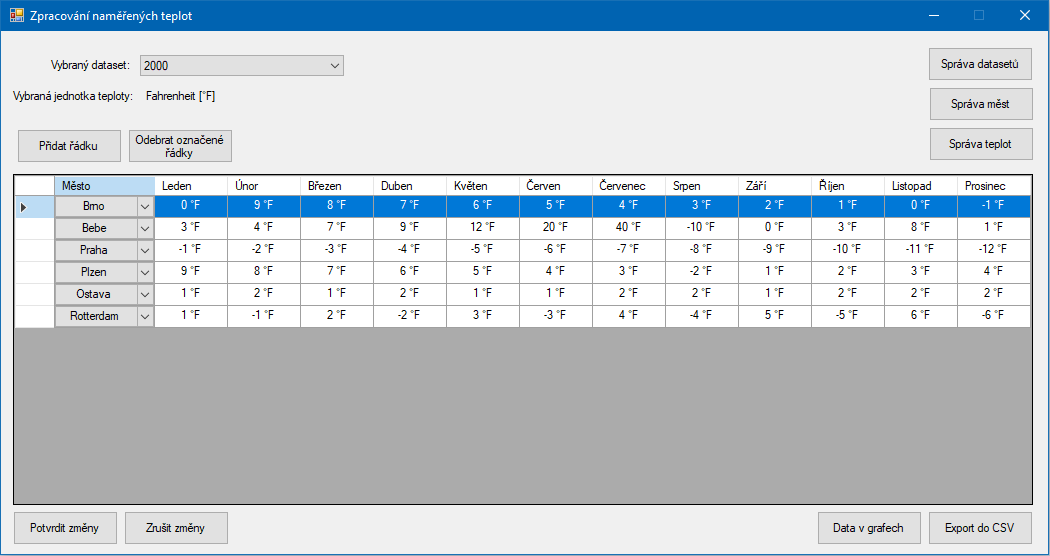
\includegraphics[width=15cm]{img/main_window.png}
	\caption{Hlavní okno}
	\label{fig:main_window}	
\end{figure}
\newpage
\subsection{Správa měst}
V okně pro správu měst se nachází tabulka se všemi názvy měst. Pro přidání nového záznamu stačí kliknout na tlačítko "\textbf{Přidat řádku}". Odebírání řádek funguje stejně jako v hlavním okně. Vzhled okna pro správu měst lze vidět na obrázku \ref{fig:manage_cities}.

Po upravení jakéhokoliv záznamu je potřeba změny uložit pomocí tlačítka "\textbf{Potvrdit změny}".
\begin{figure}[h!]
	\centering
	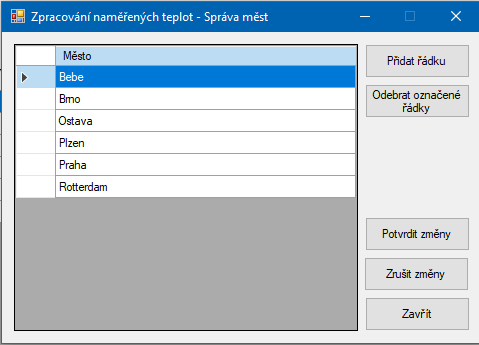
\includegraphics[width=10cm]{img/manage_cities.png}
	\caption{Správa měst}
	\label{fig:manage_cities}
\end{figure}
\newpage
\subsection{Správa jednotek teplot}
V okně pro správu jednotek teplot se nachází tabulka se dvěma sloupci. První sloupec obsahuje název jednotky teploty a druhý sloupec obsahuje symbol jednotky teploty. Přidávání / odebírání funguje stejně jako u okna pro správu měst. Vzhled okna pro správu jednotek teplot lze vidět na obrázku \ref{fig:manage_measures}.
\begin{figure}[h!]
	\centering
	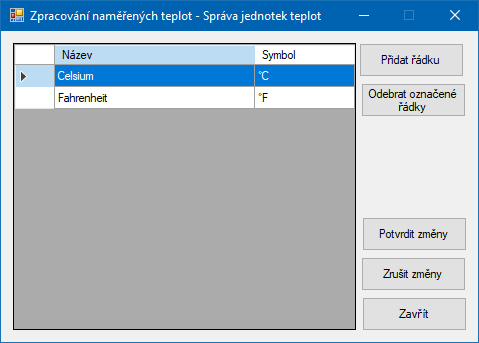
\includegraphics[width=10cm]{img/manage_measures.png}
	\caption{Správa jednotek teplot}
	\label{fig:manage_measures}
\end{figure}

\subsection{Správa datasetů}
V okně pro správu datasetů se nachází tabulka se dvěma sloupci. První sloupec obsahuje název datasetu a druhý sloupec obsahuje jednotku teploty, která bude použita pro všechny záznamy v datasetu. Přidávání / odebírání funguje stejně jako u okna pro správu měst. Vzhled okna pro správu datasetů lze vidět na obrázku \ref{fig:manage_datasets}.
\begin{figure}[h!]
	\centering
	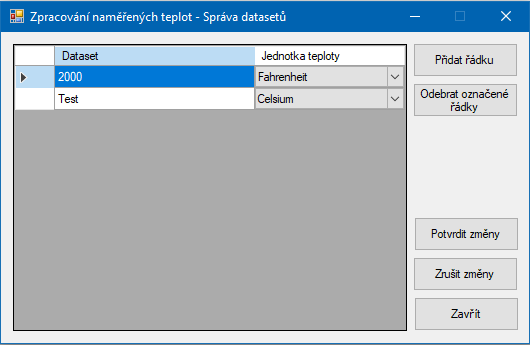
\includegraphics[width=10cm]{img/manage_datasets.png}
	\caption{Správa datasetů}
	\label{fig:manage_datasets}
\end{figure}

\subsection{Okno s grafy}
V tomto okně lze zobrazit různé typy grafů. Vzhled okna lze vidět na obrázku \ref{fig:graph_window}. 

V aplikaci jsou aktuálně definované 3 typy grafů, které se vybírají pomocí selectu s názvem "\textbf{Vybraný graf}":
\begin{itemize}
\item Průměrná teplota ve všech městech po měsíci v daný rok. 
\item Porovnání teplot více měst po měsících v daný rok.
\item Teplota ve městech za měsíc v daný rok.
\end{itemize}

Následně se v selectu s názvem "\textbf{Vybraný dataset}" zvolí dataset, který bude vizualizován. Některé typy grafů potřebují k vyobrazení dodatečná data. Tyto data se zobrazí v listboxu na pravé straně okna. Po zvolení některý možnosti (i více možností v některých případech) v tomto listboxu se zobrazí výsledný graf ve středu okna.

\newpage
\begin{figure}[h!]
	\centering
	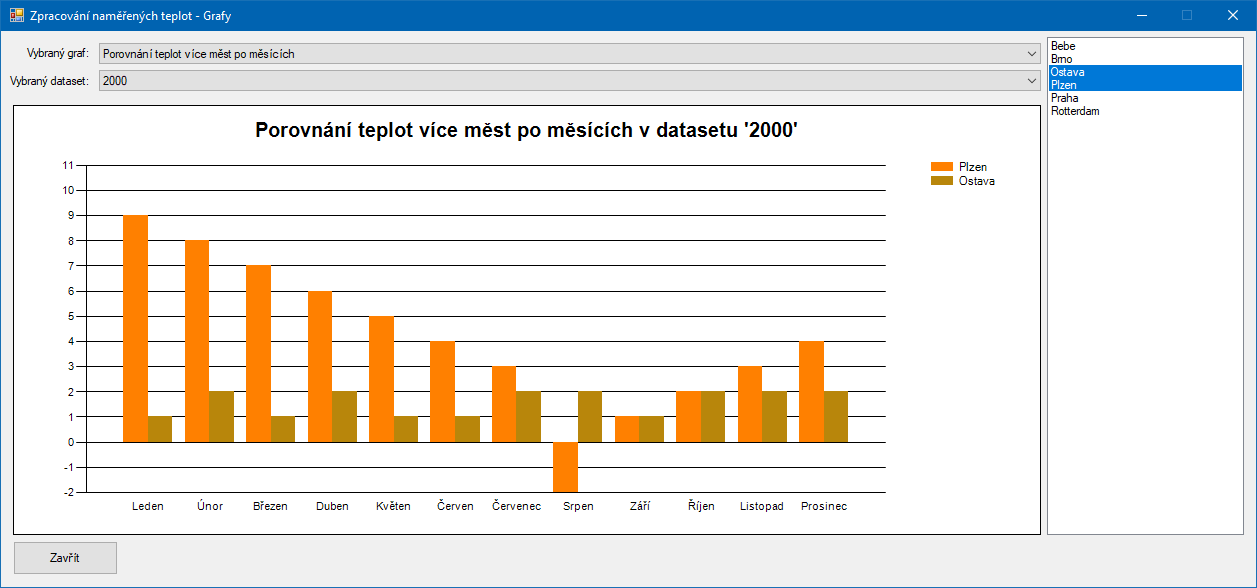
\includegraphics[width=15cm]{img/graph_window.png}
	\caption{Okno s grafy}
	\label{fig:graph_window}
\end{figure}

\newpage
\section{Závěr}
Semestrální práce splňuje zadanou funkcionalitu, ale na samém začátku projektu byly zvoleny špatné technologie (například nepoužití Entity Frameworku) a díky tomu byl náročnější vývoj této aplikace. Ovládání aplikace je velice jednoduché, k provedení akce stačí většinou kliknout na dané tlačítko nebo vyplnit dané textové pole. Uživatel je schopný si sám vytvořit veškerá data (města, datasety, jednotky teploty), které lze následně použít při vytváření záznamů v datasetu. V aplikaci je také možné si zadaná data vizualizovat v grafech.

Při testování se nevyskytly žádné chyby, které by měli zásádní vliv na funkčnost aplikace. Testovány byly především všechny možné vstupní znaky při zadávání teploty v daném měsíci a také správné chování při mazání datasetů z databáze.

\newpage
\setcounter{section}{0}
\renewcommand{\thesection}{\Alph{section}}
\section{Programátorský deník}
\begin{table}[h!]
  \begin{center}

\begin{tabular}{| cp{10cm} |c | c |}
\hline
  \textbf{Datum} & \textbf{Náplň práce} & \textbf{Strávený čas [h]}\\
\hline
4.2.2020 & Vytvoření řešení a dvou projektů (data + gui). & 1\\
\hline
27.3.2020 & Zprovoznění databáze + získávání dat & 3 \\
& Načítání dat z databáze do gui elementu & 1 \\
& Vytvořeny eventy na validaci polí v datasetu & 1 \\
& Přidávání řádků s custom buňkama do datasetu & 1 \\
\hline
3.4.2020 & Správa tabulky City v novém okně (zatím bez pushování změn). & 3 \\
& Úprava hlavního okna (tlačítka, automatické nahrání dat do datasetu) & 2 \\
\hline
10.4.2020 & Pushování změn v tabulce City - mazání / přidávání + kontroly. & 1 \\
& Správa tabulky Record (zatím bez pushování změn). &1 \\
& Správa tabulky Dataset (i s pushováním). & 3 \\
& Správa teplot v novém okně (bez pushování). & 1 \\
& Zvětšení buněk pro měsíce + jednotka teploty zobrazena jako label. & 1 \\
\hline
11.4.2020 & Bugfix správy dat (ukládání, mazání, update) v databázi. & 1 \\
& Správa teplot v novém okně (pushování). & 1 \\
& Bugfix mazání datasetů. & 1 \\
& Zobrazení jednotky teploty u buněk měsíců. & 1 \\
\hline
14.4.2020 & Správa recordů (pushování). & 4 \\
& Drag \& Drop recordů - změna pořadí. & 1 \\
& Export dat do csv. & 1 \\
& Validace hodnot buněk v record datagridview. & 4 \\
\hline
18.4.2020 & Kontrola, zda se aktuální dataset změnil či ne při přehazování datasetů / exportování do csv. & 1 \\
& Vytvoření 2 (bez porovnávání měst mezi sebou) grafů. & 3 \\
& Vytvoření grafu pro porovnávání měst mezi sebou + implementace staženého checkboxComboboxu. & 3 \\
\hline
9.5.2020 & Komentáře & 2 \\
& Menší restrukturalizace projektu & 2 \\
\hline
21.5.2020 & Opravení projektu (nefungující SqlClient) & 2 \\
& Dokumentace & 3 \\
\hline
& \textbf{Celkový čas} & \textbf{49} \\
\hline
\end{tabular}
\end{center}
\end{table}

\end{document}